\documentclass{article}
\usepackage{amsmath,amssymb,amsthm,latexsym,paralist,url}
\usepackage[margin=1in]{geometry}
\usepackage{tikz}
\usepackage{graphicx}
\usetikzlibrary{arrows,automata}
\usepackage{csquotes}

\theoremstyle{definition}
\newtheorem{problem}{Problem}
\newtheorem*{solution}{Solution}
\newtheorem*{resources}{Resources}


\newcommand{\honor}{\noindent \textbf{Aggie Honor Statement: }On my honor as an Aggie, I have neither
  given nor received any unauthorized aid on any portion of the academic work included in this assignment.
}

 
\newcommand{\checklist}{\noindent\textbf{Checklist:}
Did you...
\begin{compactenum}
\item abide by the Aggie Honor Code?
\item solve all problems?
\item start a new page for each problem?
\item show your work clearly?
\item type your solution?
\item submit a PDF to gradescope and correctly assign problems to pages?
\end{compactenum}
}

\newcommand{\problemset}[1]{\begin{center}\textbf{Homework #1}\end{center}}
\newcommand{\duedate}[1]{\begin{quote}\textbf{Due: #1} on gradescope (\url{gradescope.com}). \\You must show your work in order to receive credit.\end{quote}}

%%% CONSTANTS
\newcommand{\mysemester}[0]{Spring 2018}
\newcommand{\mysectionnumber}[0]{501,502}
\newcommand{\myname}[0]{Hunter Cleary}
\newcommand{\homeworknumber}[0]{8}

%%% HEADERS & FOOTERS
\usepackage{fancyhdr} % This should be set AFTER setting up the page geometry
\pagestyle{fancy} % options: empty , plain , fancy
\renewcommand{\headrulewidth}{0pt} % customise the layout...
\lhead{CSCE 222-\mysectionnumber}\chead{Homework \homeworknumber}\rhead{\myname}
\lfoot{}\cfoot{\thepage}\rfoot{}

\title{CSCE 222: Discrete Structures for Computing\\Section \mysectionnumber\\\mysemester}
\author{\myname}
\date{}

\begin{document}

\maketitle
\problemset{\homeworknumber}
\duedate{26 March 2018 (Monday) before 11:59 p.m.}
\bigskip

\honor
\bigskip

\checklist

% functions
\begin{problem} (35 points)\\
Show for each pair of functions that $f(x)$ is $O(g(x))$ and $g(x)$ is $O(f(x))$.
\begin{compactenum}
\item $f(x) = 4x+7$, $g(x) = x$
\item $f(x) = -7x^2 - 2x + 3$, $g(x) = x^2$
\item $\displaystyle f(x) = \frac{7x^3 + 8x^2 - 3x - 7}{2x^2 + 5x + 8}$, $g(x) = x$
\item $f(x) = \log (x^2+1)$, $g(x) = \log x$
\item $f(x) = \log_{10} x$, $g(x) = \log_2 x$
\end{compactenum}
\end{problem}

\begin{solution}\ \\
\begin{compactenum}


\item $f(x) = 4x+7 , g(x) = x$\ \\
$4x+7 <= cx , x>k$\ \\
$4x <= cx - 7 $\ \\
$4 <= c-7$\ \\
$4<=11-7$\ $c=11,k=1$\ \\
$ x <= 4x + 7 , c=4 , k=1 $\ \\
\therefore \  $f(x) is O(g(x)) and g(x) is O(f(x))$\ \\

\item $f(x) = -7x^2 - 2x + 3$, $g(x) = x^2$\ \\
$-7x^2 - 2x + 3$\ \\
$7x^2 - 2x + 3 <= x^2 , c=1, k=0$\ \\
$x^2 <= x^2 , c=1, k=0$\ \\
\therefore \  $f(x) is O(g(x)) and g(x) is O(f(x))$\ \\

\item $\displaystyle f(x) = \frac{7x^3 + 8x^2 - 3x - 7}{2x^2 + 5x + 8}$, $g(x) = x$\ \\
$\displaystyle \frac{7x^3 + 8x^2 - 3x - 7}{2x^2 + 5x + 8} <= x ,c= 7/2 , k= 1$\ \\
$x <= x, c=1 , k=1$\ \\
\therefore \  $f(x) is O(g(x)) and g(x) is O(f(x))$\ \\

\item $f(x) = \log (x^2+1)$, $g(x) = \log x$\ \\
$\log (x^2+1) <= 2 \log (x), c = 2, k = 1$\ \\
$\log x <= \log x , c = 1, k = 1$\ \\
\therefore \  $f(x) is O(g(x)) and g(x) is O(f(x))$\ \\

\item $f(x) = \log_{10} x$, $g(x) = \log_2 x$\ \\
$ \log_{10} x <= \log x, c = 1, k = 1$\ \\
$ \log_{2} x <= \log x, c =1, k = 1$\ \\
\therefore \  $f(x) is O(g(x)) and g(x) is O(f(x))$\ \\

\end{compactenum}
\end{solution}
%\newpage
\ \\
% algorithms
\begin{problem}(33 points)\\ 
Show that $1^k + 2^k + \cdots + n^k$ is $O(n^{k+1})$.
\end{problem}

\begin{solution}\ \\
$1^k + 2^k + \cdots + n^k$\ \\
$1^k + 2^k + \cdots + n^k <= n^k + n^k \cdots +n^k $\ \\
$n^k + n^k \cdots +n^k = n*n^k$\ \\
$n*n^k = n^k+1$\ \\
\therefore \ $1^k + 2^k + \cdots + n^k$ is $O(n^{k+1})$
\end{solution}

\newpage
\ \\ \ \\
%algorithms
\begin{problem} (32 points)\\
Let $H_n$ be the $n$-th \textbf{harmonic number}
$$H_n = 1 + \frac{1}{2} + \frac{1}{3} + \cdots + \frac{1}{n}.$$
Show that $H_n$ is $O(\log n)$.
\ \\
\ \\
Hint: First establish the inequality $$\sum_{j=2}^n \frac{1}{j} < \int_1^n \frac{1}{x}dx$$ by showing that the sum of the areas of the rectangles of height $1/j$ with base from $j-1$ to $j$, for $j=2,3,\ldots,n$, is less than the area under the curve $y=1/x$ from 2 to $n$.
%There's another way... maybe easier.
\end{problem}
\begin{solution}\ \\
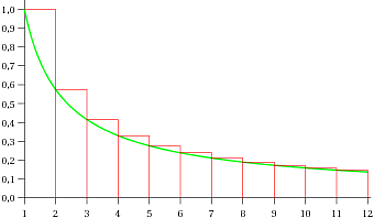
\includegraphics[width=\textwidth ,height=\textheight,keepaspectratio]{SpHUQ.png}\ \\
The nth harmonic decreases at a rate faster than that of O(logn).\ \\
\therefore \ $H_n$ is $O(\log n)$
\end{solution}




\end{document}
